\documentclass[a4paper,10pt]{report}
\usepackage{fontenc}
\usepackage{graphicx} % to include images
\usepackage[top=1in,bottom=1in,left=1in,right=1in]{geometry} % to set page margins 
\usepackage{url} % to include url's
\usepackage{color} % to include colors
\usepackage{fancyhdr} % for header and footer






\begin{document}
\begin{titlepage}
\centering
\vfill
\textbf{\Huge{\textcolor{cyan}{\rule{\textwidth}{12pt}}\\{EEP773
\linebreak
\\Telecom Software\vskip0.5cm Lab}}} \vskip0.5cm
{\textcolor{cyan}{\rule{\textwidth}{12pt}}}\\
\vspace{2cm}
\Large{\textbf{ASSIGNMENT No. 09\\Report} \vskip 1cm
}
\vskip2cm
\Large{\textbf{\\Debesh Panda\\Entry No: 2014JTM2499}}
\\Sept. 24th,2014\\
\vskip3cm
\begin{figure}[ht]
 \centering

\includegraphics[scale=0.2]{./logo.png}
 % logo.png: 899x935 pixel, 96dpi, 23.78x24.74 cm, bb=0 0 674 701
\end{figure}

{\textbf{
Indian Institute of Technology, Delhi}}
\vfill
\end{titlepage}

\tableofcontents
\pagebreak
\listoffigures


\pagebreak
\chapter{Problem Statement}
\section{For determining behaviour of users}
\begin{itemize}
 \item Python is useful in data analysis and string manipulation. 
 \item n this assignment, you are supposed to analyze a data file on the basis of different 
emoticons and words that reflect emotions. 
\item Content file is given in the below format
\item A dictionary is also given to predict the meaning of emoticons and some specific
words.
\item Depending on this dictionary, you have to count the number of emoticons and words
that are there in the dictionary.
\item Finally output the behavior of user.
\item Also output percentage of different behaviors that are found in the dictionary.
\end{itemize}

\section{Bonus marks}
Add method to include more contents in the database.
\newpage
\chapter{Assumption}
\begin{itemize}
  \item The content file will be passed through commandlind arguement.
 \item For any user frequecy of different modes used is calculated and maximum is assumed to be his behavior
 
 
\end{itemize}
\newpage
\chapter{Logic Implemented}
\section{Determining behavior of users}
\begin{itemize}
 \item Each line of the text file is traveresed through for loop then each word is again traversed in the line and checked for the emoticons.
 \item If a particular emoticon is matched then the correponding mode is updated in an array and this is done for each user and the mode of the user is determined based upon the maximum count of each mood of the users
\end{itemize}


\section{Calculating the percentage}
The percentage of each mood is calculated based upon the mood count that was counted earlier in this program.




\newpage
\chapter{Output Snapshot}
\begin{figure}[ht]
 \centering
 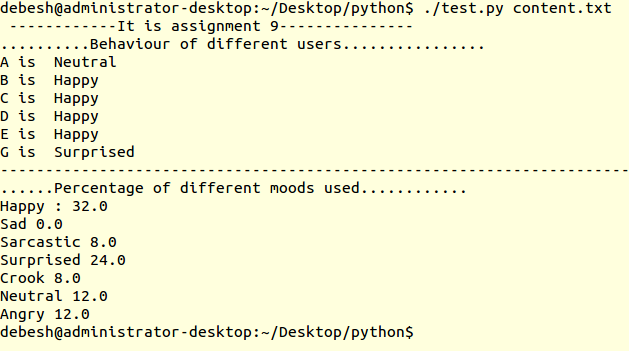
\includegraphics[scale=0.8]{./Selection_006.png}
 % Selection_006.png: 629x351 pixel, 72dpi, 22.19x12.38 cm, bb=0 0 629 351
 \caption{output}
\end{figure}












\newpage % new page starts
\begin{thebibliography}{widestlabel} % bibliography beginning
\bibitem{}\url{https://developers.google.com/edu/python/}          %\bibitem is for bibliography item and \url to write url's
\bibitem{}\url{https://docs.python.org/2/tutorial/}
\bibitem{}\url{http://www.tutorialspoint.com/python/}


\end{thebibliography} % ends the bibliography



\end{document}



